\chapter{\sffamily Managing a rugby match}

{\bfseries\sffamily Concept.} Building a toy model simulation of a rugby match whose outcome can be manipulated through correctly-timed player substitutions and game management decisions. The dexetera state manipulation framework we have built around the stochadex can meet these requirements, and a dashboard can be created for user interaction. All this combines together to make a simple dashboard game, which we call: `trywizard'. For the mathematically-inclined, this chapter will motivate the construction of a specific modelling framework for rugby match simulation. For the programmers, the public Git repository for the code described in this chapter can be found here: \href{https://github.com/umbralcalc/trywizard}{https://github.com/umbralcalc/trywizard}.

\section{\sffamily Designing the event simulation engine}

Since the basic state manipulation framework and simulation engine will run using \href{https://github.com/umbralcalc/dexetera}{dexetera}, the mathematical novelties in this project are all in the design of the rugby match model itself. And, as ever, we're not especially keen on spending a lot of time doing detailed data analysis to come up with the most realistic values for the parameters that are dreamed up here. Even though this would also be interesting.\footnote{One could do this data analysis, for instance, by scraping player-level performance data from one of the excellent websites that collect live commentary data such as \href{https://www.rugbypass.com/}{rugbypass.com} or \href{https://www.espn.co.uk/rugby/}{espn.co.uk/rugby}.}

Let's begin by specifying an appropriate state space to live in when simulating a rugby match. It is important at this level that events are defined in quite broadly applicable terms, as it will define the state space available to our stochastic sampler and hence the simulated game will never be allowed to exist outside of it. It seems reasonable to characterise a rugby union match by the following set of states: {\sf Penalty}, {\sf Free Kick} (the punitive states); {\sf Penalty Goal}, {\sf Drop Goal}, {\sf Try} (the scoring states); {\sf Kickoff}, {\sf Kick Phase}, {\sf Run Phase}, {\sf Knock-on}, {\sf Scrum}, {\sf Lineout}, {\sf Maul} and {\sf Ruck} (the general play states). Using this set of states, in Fig.~\ref{fig:event-graph} we have summarised our approach to match state transitions into a single event graph. In order to capture the fully detailed range of events that are possible in a real-world match, we've needed to be a little imaginative in how we define the kinds of state transitions which occur. In other words; it's fair to say that our simplified model here represents just a subset of states that a real rugby match could exist in.

\begin{figure}[h]
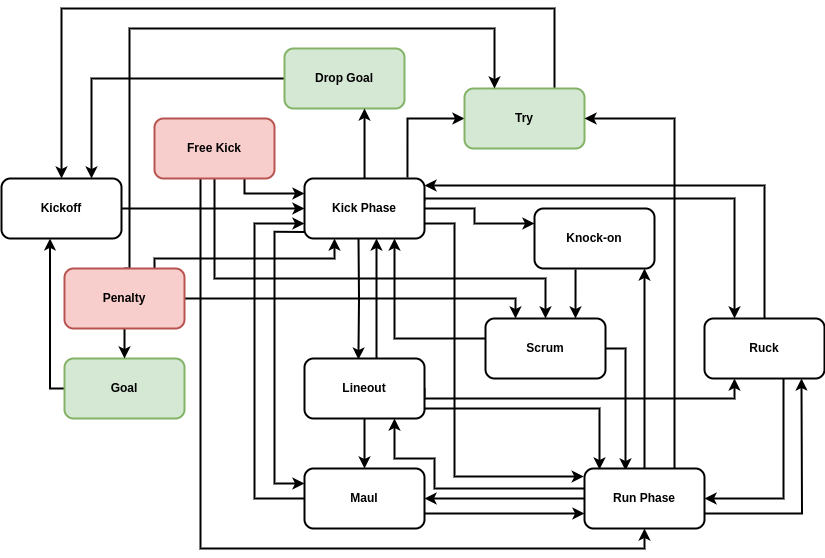
\includegraphics[width=14cm]{images/trywizard-event-graph.drawio.png}
\caption{Simplified event graph of a rugby union match.}
\label{fig:event-graph}
\end{figure}

In addition to occupying some state in the event graph, the state of a rugby match must also include a binary `possession' element which encodes which team has the ball at any moment. We should also include the 2-dimensional pitch location of the ball as an element of the match state in order to get a better sense of how likely some state transitions are, e.g., when playing on the edge of the pitch near the touchline it's clearly more likely that a {\sf Run Phase} is going to result in a {\sf Lineout} than if the state is currently in the centre of the pitch. To add even more detail; in the next section we will introduce states for each player.

Since a rugby match exists in continuous time, it is natural to choose a continuous-time event-based simulation model for our game engine. As we have discussed in previous chapters already, this means we will be characterising transition probabilities of the event graph in Fig.~\ref{fig:event-graph} by ratios of event rates in time. Recalling our notation in previous chapters, if we consider the current state vector of the match $X_{\sf t}$, we can start by assigning each transition ${\sf a}\rightarrow {\sf b}$ on the event graph an associated expected rate of occurance $\lambda_{{\sf a}\rightarrow {\sf b}}$ which is defined in units of continuous time, e.g., seconds. In addition to the transitions displayed on the graph, we can add a `possession change transition'; where the possession of the ball in play moves to the opposing team. This transition may occur while the match is also in any of the white-coloured states on the graph (apart from {\sf Knock-on} which determines a possession change immediately through a {\sf Scrum}) and let's assign this a state, parameter and timestep-dependent expected rate of occurance $\lambda_{\rm pos}(X_{\sf t}, z, {\sf t})$.

Based on our dicussion above, an appropriate encoding for the overall game state at timestep index ${\sf t}$ could be a state vector $X_{{\sf t}}$ whose elements are
%%
\begin{align}
X^0_{{\sf t}}&=\begin{cases} 0 & \text{Match State} = \text{{\sf Penalty}}\\ 1 & \text{Match State} = \text{{\sf Free Kick}} \\ \dots & \end{cases} \\
X^1_{{\sf t}}&=\begin{cases} 0 & \text{Possession} = \text{{\sf Home Team}}\\ 1 & \text{Possession} = \text{{\sf Away Team}} \end{cases} \,.
\end{align}
%%
But how does this overall game state connect to the event rates? The probabilistic answer is quite straightforward. If the probability of the match state being $X^0_{{\sf t}}={\sf a}$ at timestep ${\sf t}$ is written as $P^0_{{\sf t}}({\sf a})$, then the probability of $X^0_{{\sf t}+1}={\sf b}$ in the following timestep is
%%
\begin{align}
P^0_{{\sf t}+1}({\sf b}) = \frac{\frac{1}{\tau}P^0_{{\sf t}}({\sf b})+\sum_{\forall {\sf a}\neq {\sf b}}\lambda_{{\sf a}\rightarrow {\sf b}}{\cal T}_{{\sf a}\rightarrow {\sf b}}(X_{\sf t}, z, {\sf t})P^0_{{\sf t}}({\sf a})}{\big[ \frac{1}{\tau} + \sum_{\forall {\sf a}\neq {\sf b}}\lambda_{{\sf a}\rightarrow {\sf b}} {\cal T}_{{\sf a}\rightarrow {\sf b}}(X_{\sf t}, z, {\sf t})\big]} \label{eq:match-state-transition-probs}\,,
\end{align}
%%
where $\forall {\sf a} \neq {\sf b}$ in the summation indicates that all the available transitions from ${\sf a}$ to ${\sf b}$, where ${\sf a}\neq {\sf b}$, should be summed over and ${\cal T}_{{\sf a}\rightarrow {\sf b}}(X_{\sf t}, z, {\sf t})$ is a time, parameter and state-dependent transition probability that is determined by the playing tactics of each team as well as the general likelihoods of gameplay which are expected from a real rugby match. Note that in the expression above, we have also defined $\tau$ as a timescale short enough such that no transition is likely to occur during that interval. An equivalent to Eq.~(\ref{eq:match-state-transition-probs}) should also apply to the possession change transition rate, i.e., the probability that the {\sf Home Team} has possession $P^1_{{\sf t}}$ at time ${\sf t}$ evolves according to
%%
\begin{align}
P^1_{{\sf t}+1} = \frac{ \frac{1}{\tau}P^1_{{\sf t}} + \lambda_{\rm pos}(X_{\sf t}, z, {\sf t}) (1-P^1_{{\sf t}})}{\big[ \frac{1}{\tau} + \lambda_{\rm pos}(X_{\sf t}, z, {\sf t})\big]} \label{eq:possession-change-probs}\,.
\end{align}
%%

Before we move on to other details, it's quite important to recognise that because our process is defined in continuous time, the possession change rate may well vary continuously (this will be especially true when we talk about, e.g., player fatigue). Hence, Eq.~(\ref{eq:match-state-transition-probs}) is only an \emph{approximation} of the true underlying dynamics that we are trying to simulate --- and this approximation will only be accurate if $\tau$ is small. The reader may recall that we discussed this same issue from the point of view of simulating time-inhomogeneous Poisson processes with the rejection method when we were building the stochadex in an earlier chapter. 

While these match state transitions and possession changes are taking place, we also need to come up with a model for how the ball location $L_{{\sf t}}$ changes during the course of a game, and as a function of the current game state. Note that, because the ball location is a part of the overall game state, it will be included as information contained within some elements of $X_{{\sf t}}$ as well. To make this explicit, we can simply set $X^2_{{\sf t}}=L^{\rm lon}_{{\sf t}}$ and $X^3_{{\sf t}}=L^{\rm lat}_{{\sf t}}$ --- where $L^{\rm lon}_{{\sf t}}$ denotes the longitudinal component (lengthwise along the pitch) and $L^{\rm lat}_{{\sf t}}$ denotes the lateral component (widthwise across the pitch). If we associate every state on the event graph with a single change in spatial location of the ball on the pitch, we then need to construct a process which makes `jumps' in 2-dimensional space each time a state transition occurs. To keep things simple and intuitive, we will say that movements of the ball are only allowed to occur during either a {\sf Run Phase} or a {\sf Kick Phase}. 

In the case of a {\sf Run Phase}, let's choose the longitudinal component of the ball location $L^{\rm lon}_{{\sf t}}$ to be updated by the difference between samples drawn from two exponential distributions (one associated to each team). Hence, the probability density $P_{{\sf t}+1}(\ell )$ of $L^{\rm lon}_{{\sf t}+1}-L^{\rm lon}_{{\sf t}}=\ell$, evolves according to
%%
\begin{align}
P_{{\sf t}+1}(\ell ) = \int^\infty_0 {\rm d}\ell'\, {\sf ExponentialPDF}(\ell + \ell'; a_{\rm run}){\sf ExponentialPDF}(\ell'; d_{\rm run}) \label{eq:longitudinal-motion-rugby} \,,
\end{align}
%%
where $a_{\rm run}$ and $d_{\rm run}$ are the exponential distribution scale parameters for an attacking and defending player, respectively, and we have chosen positive values of $\ell$ to be aligned with the forward direction for the attacking team. We shall elaborate on where $a_{\rm run}$ and $d_{\rm run}$ come from when we discuss associating events for player abilities in due course. If we now consider lateral component of the ball location $L^{\rm lat}_{{\sf t}}$ during a {\sf Run Phase}; it makes sense that this wouldn't be affected much by either team within the scope of detail in this first version of our model. Hence, the probability density $P_{{\sf t}+1}(w)$ of $L^{\rm lat}_{{\sf t}+1}-L^{\rm lat}_{{\sf t}}=w$ can just be updated like so
%%
\begin{align}
P_{{\sf t}+1}(w) = {\sf NormalPDF}(w; 0, \sigma_{\rm run}^2) \label{eq:lateral-motion-rugby} \,,
\end{align}
%%
where $\sigma_{\rm run}$ is the typical jump in lateral motion (the standard deviation parameter of the normal distribution).

Turning our attention to the {\sf Kick Phase}; the longitudinal component is only realistically controlled by the attacking team. There's also an angular component to this motion which is associated to the direction that the kicker is orientating their kick. Let's begin by defining the chosen angle $\theta$ of the attacking team player who is kicking (where straight ahead is defined as $\theta = 0$) such that
%%
\begin{align}
L^{\rm lon}_{{\sf t}+1}-L^{\rm lon}_{{\sf t}}&=\ell \cos \theta + w \sin \theta \\
L^{\rm lat}_{{\sf t}+1}-L^{\rm lat}_{{\sf t}}&=\ell \sin \theta + w \cos \theta \,.
\end{align} 
%%
Therefore, the probability density of $P_{{\sf t}+1}(\ell )$ will evolve according to
%%
\begin{align}
P_{{\sf t}+1}(\ell ) = {\sf ExponentialPDF}(\ell; a_{\rm kick}) \label{eq:longitudinal-motion-rugby-kicking} \,,
\end{align}
%%
where $a_{\rm kick}$ this time is the exponential scale parameter for the attacking team player who is kicking. Similarly, the lateral component for a {\sf Kick Phase} is only going to be controlled by the accuracy of the kicker. Therefore, the corresponding update to the probability density is
%%
\begin{align}
P_{{\sf t}+1}(w) = {\sf NormalPDF}(w;0, \sigma_{\rm kick}^2) \label{eq:lateral-motion-rugby-kicking} \,,
\end{align}
%%
with a standard deviation $\sigma_{\rm kick}$, and its interpretation now being the accuracy of the kicker.

\section{\sffamily Associating events to player states and abilities}

In the last section we introduced a continuous-time event-based simulation model for a rugby union match. In this section we are going to add more detail into this model by inventing how to associate specific player states and abilities to the event rates of the simulation. Before continuing, we want to reiterate that this model is entirely made up and, while we hope it illustrates some interesting mathematical modelling ideas in the context of rugby, there's no particular reason why a statistical inference with a reliable dataset should prefer our model to others which may exist.

In Fig.~\ref{fig:player-abilities} we began by separating playing positions on the rugby field into their usual descriptions and then associating each player type with a short list of simplified attributes. Our model is then to associate a player with an `possession attacking' and `possession defending' ability which corresponds to each of their attributes. For example, a Front Row Forward will have 8 abilities associated to them: 2 for each of their {\sf Scrum}, {\sf Lineout}, {\sf Ruck} and {\sf Maul} attributes.

\begin{figure}[h]
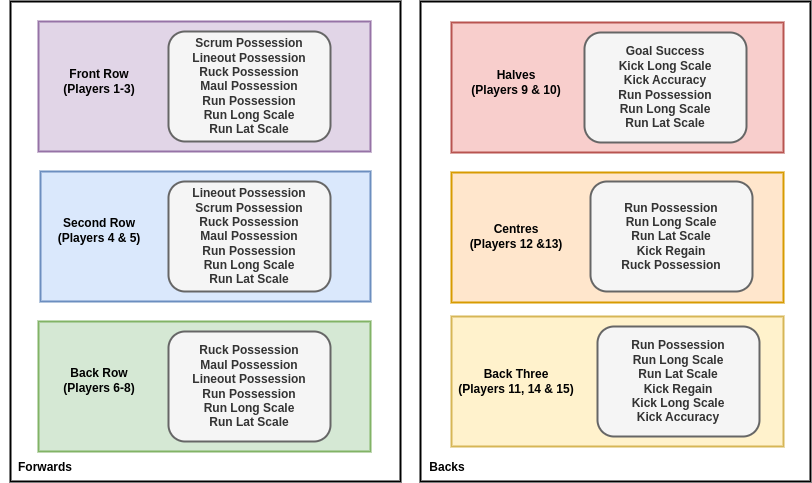
\includegraphics[width=15cm]{images/rugby-player-abilities.drawio.png}
\caption{Associated playing abilities for each position type.}
\label{fig:player-abilities}
\end{figure}

Let's now say that $z$ contains all of these parameters for all of the players on both sides, and also whether or not each player is actively playing or on the bench. With this information, and the knowledge of which team is in possession from $X^1_{\sf t}$, it should be simple to create a vector-valued function $a_{\rm pos}(X_{\sf t}, z)$ which returns all of the posession attacking attributes that are associated to match state $X^0_{\sf t}$ and an analogous one $d_{\rm pos}(X_{\sf t}, z)$ for the possession defending attributes. The dependencies of these functions on the ball possession state $X^1_{\sf t}$ comes from the fact that when, e.g., the {\sf Home Team} has possession of the ball it will be their possession attacking attributes that are returned by $a_{\rm pos}(X_{\sf t}, z)$ and the {\sf Away Team}'s possession defending attributes that are returned by $d_{\rm pos}(X_{\sf t}, z)$.

In order to model the effect of player fatigue over the course of a match, we can add some vectors of player fatigue values $f$ and times at which each player started playing $t_{\rm start}$ into the collection of parameters that are contained within $z$. These new parameters can then be used to define a formula for the decline of each attribute over the course of a match. Let's assign these declining values to be part of the overall match state like so
%%
\begin{align}
X^j_{\sf t} &= a^j_{\rm pos}(X_{\sf t}, z)e^{-f^j[t({\sf t})-t^j_{\rm start}]} \label{eq:att-player-fatigue} \\
X^k_{\sf t} &= d^k_{\rm pos}(X_{\sf t}, z)e^{-f^k[t({\sf t})-t^k_{\rm start}]} \label{eq:def-player-fatigue} \,,
\end{align}
%%
where the $j$ and $k$ each index the range of indices in the overall match state which correspond to the attacking and defending team player states, respectively.

So how does each player affect the events of a match? In our model, we would argue that players should be able to directly influence the possession change rate $\lambda_{\rm pos}(X_{\sf t}, z, {\sf t})$ through a balance of attacking and defensive attributes in the following relation
%%
\begin{align}
\lambda_{\rm pos}(X_{\sf t}, z, {\sf t}) &= \frac{\lambda^*_{\rm pos}\sum_{\forall j}X^j_{{\sf t}}}{\sum_{\forall j}X^j_{{\sf t}} + \sum_{\forall k}X^k_{{\sf t}}}\,,
\end{align}
%%
where $\lambda^*_{\rm pos}$ is the maximum rate that is physically possible and the $\forall j$ and $\forall k$ in the summations indicate summing over all attacking and defending player attributes, respectively. In addition to this possession change influence, players who have {\sf Run Phase} and {\sf Kick Phase} attributes may affect the gain in distance (and accuracy in the case of {\sf Kick Phase}) that each state translates to on the pitch. 

Let's first describe how we intend the {\sf Run Phase} to work. Every time the match state transitions into a {\sf Run Phase}, an individual player on the attacking side is chosen at random (uniformally across the team\footnote{This uniform sampling could be refined later to associate sampling probabilities with game state and player roles.}) to be the the nominal `attacker'. At the same time, an individual player on the defending side is chosen at random (again, uniformally across the team) to be the the nominal `defender'. Once these players have been chosen (and hence the $a_{\rm run}$ and $d_{\rm run}$ parameters have been determined), the longitudinal motion update we described in Eq.~(\ref{eq:longitudinal-motion-rugby}) can then be applied. Note that the $a_{\rm run}$ and $d_{\rm run}$ parameters should also receive a fatigue decrement depending on the time that each player has remained on the pitch, much like the exponential factors we applied in Eqs.~(\ref{eq:att-player-fatigue}) and~(\ref{eq:def-player-fatigue}).

Finally, we turn or attention to the mechanics of a {\sf Kick Phase}. For tactical kicking in the middle of play, this operates in a similar way as a {\sf Run Phase}; one of the players on the attacking side (the side in possession of the ball) is chosen at random (uniformally) and their $a_{\rm kick}$ and $\sigma_{\rm kick}$ attributes are used in Eqs.~(\ref{eq:longitudinal-motion-rugby-kicking}) and~(\ref{eq:lateral-motion-rugby-kicking}) to update the position of the ball. In the specific case of {\sf Goal} kicking from a {\sf Penalty}, the designated place kicker on each side also uses their same {\sf Kick Phase} attributes to determine the success/failure of the kick at the posts.

\section{\sffamily Deciding on managerial actions}

So how does managing a rugby match map to taking actions with our formalism? We have to figure out what sorts of managerial actions ${\cal A}_{{\sf t}+1}$ are parametric in nature (affecting $z$) and if any directly act on the state of the system itself (affecting $X_{{\sf t}+1}$). Let's jump straight to the answer to the second question; it doesn't seem like there is any situation where the overall match state $X_{\sf t}$ itself is directly changed by a managerial action, so we will be using only parametric actions in this chapter.

Our model structure would suggest that the only way in which a manager can influence the state of a match is through modifying the parameters which are used by the $a_{\rm pos}(X_{\sf t},z)$, $d_{\rm pos}(X_{\sf t},z)$ or ${\cal T}_{{\sf a}\rightarrow {\sf b}}(X_{\sf t},z,{\sf t})$ functions. In the case of the possession attacking and defending attributes $a_{\rm pos}(X_{\sf t},z)$ and $d_{\rm pos}(X_{\sf t},z)$, a parametric action that the manager can perform would be to modify which players are actively playing through substitutions. To indicate that this underlying data may change, we can promote $z$ to its actionable, time-dependent version $Z_{{\sf t}}$ such that the functions now become $a_{\rm pos}(X_{\sf t},Z_{\sf t})$ and $d_{\rm pos}(X_{\sf t},Z_{\sf t})$. In order to map substitutions/initial squad selections to the vector ${\cal A}_{{\sf t}+1}$, we can define the first set of 15 indices ${\cal A}_{{\sf t}+1}^i$ (where $i=0,\dots , 14$) as the player IDs chosen to be on the pitch for either the {\sf Home Team} or the {\sf Away Team}, depending on which side the manager is in charge of. If $Z_{\sf t}$ contains all of these IDs and the positions that they are allowed to play (as well as whether they are currently playing or not), then when the manager wishes to make a substitution, all that is needed is a change to ${\cal A}_{{\sf t}+1}^i$ and the parametric action function $G_{{\sf t}+1}(Z_{\sf t},{\cal A}_{{\sf t}+1})$ can be defined to make a change $Z_{\sf t}\rightarrow Z_{{\sf t}+1}$ in response to this.

But what about ${\cal T}_{{\sf a}\rightarrow {\sf b}}(X_{\sf t},Z_{\sf t},{\sf t})$? What kinds of managerial actions can change the state transition probabilities through parameters? Given that these transition probabilities mostly arise from the tactics of each team, if the tactics of either team were changed throughout the match due to managerial decisions, these actions could be mapped to ${\cal T}_{{\sf a}\rightarrow {\sf b}}(X_{\sf t},Z_{\sf t},{\sf t})$. In order for these actions to have a clear influence on the game, however, we need to specify how team tactics get translated into transition probabilities. To keep things as simple as possible, we're going to specify only two tactical `axes' on which a manager has to decide a position during each moment of the match.

The first, and perhaps more obvious, tactical decision axis to dynamically manipulate is the ratio between {\sf Kick Phase} and {\sf Run Phase} that the team chooses when it has possession of the ball, depending on what part of the pitch they are playing in. The second axis maps how aggressively a team pursues scoring tries over any other points (even when they may be on offer from a {\sf Penalty Goal}). This latter axis also only really matters for the team in possession of the ball, so we aren't planning to map out any defensive tactics in our model for now. Since both of these actions can be mapped to a single axis each, these ratios $\rho$ (each defined between $1\geq \rho \geq 0$) can populate the last two indices of the actions vector: ${\cal A}^{15}_{{\sf t}+1}$ and ${\cal A}^{16}_{{\sf t}+1}$. When either of them has been changed, this can be mapped to $Z_{{\sf t}+1}$ using the parametric action function $G_{{\sf t}+1}(Z_{\sf t},{\cal A}_{{\sf t}+1})$ and then $Z_{{\sf t}+1}$, in turn, can change the corresponding ratios between transition probabilities ${\cal T}_{{\sf a}\rightarrow {\sf b}}(X_{{\sf t}+1},Z_{{\sf t}+1},{\sf t}+1)$ when the attacking team is making these in-play decisions in the proceeding timestep.

Before moving on to the next section, there's a quick point to make about how managerial actions can affect ball locations on the pitch. In addition to the changes that we have discussed above, let's recall that the parameters $a_{\sf run}$, $d_{\sf run}$, $a_{\rm kick}$ and $\sigma_{\rm kick}$ in Eqs.~(\ref{eq:longitudinal-motion-rugby}), (\ref{eq:longitudinal-motion-rugby-kicking}) and (\ref{eq:lateral-motion-rugby-kicking}) can be indirectly determined by the manager to some extent through player selection/substitutions. So, while tactical managerial actions can change the ratios of state transitions themselves (at least while in possession of the ball), the players which are chosen in the first place (or by substitution) can have quite a significant influence on the outcome of a match.

\section{\sffamily Writing the game itself}

\begin{itemize}
\item{Show which stochadex/dexetera methods were called and how they were used to simulate the game.}
\item{Give a summary of how the dashboard backend works (diagram would help) and how this connects up to the streamlit frontend via protobuf messages.}
\end{itemize}